%%%%%%%%%%%%%%%%%%%%%%%%%%%%%%%%%%%%%%%%%
% Jacobs Landscape Poster
% LaTeX Template
% Version 1.0 (29/03/13)
%
% Created by:
% Computational Physics and Biophysics Group, Jacobs University
% https://teamwork.jacobs-university.de:8443/confluence/display/CoPandBiG/LaTeX+Poster
% 
% Further modified by:
% Nathaniel Johnston (nathaniel@njohnston.ca)
%
% This template has been downloaded from:
% http://www.LaTeXTemplates.com
%
% License:
% CC BY-NC-SA 3.0 (http://creativecommons.org/licenses/by-nc-sa/3.0/)
%
%%%%%%%%%%%%%%%%%%%%%%%%%%%%%%%%%%%%%%%%%

%----------------------------------------------------------------------------------------
%	PACKAGES AND OTHER DOCUMENT CONFIGURATIONS
%----------------------------------------------------------------------------------------

\documentclass[final]{beamer}

\usepackage[scale=1.24]{beamerposter} % Use the beamerposter package for laying out the poster
\usepackage{wrapfig}

\usetheme{confposter} % Use the confposter theme supplied with this template



%-----------------------------------------------------------
% Define the column widths and overall poster size
% To set effective sepwid, onecolwid and twocolwid values, first choose how many columns you want and how much separation you want between columns
% In this template, the separation width chosen is 0.024 of the paper width and a 4-column layout
% onecolwid should therefore be (1-(# of columns+1)*sepwid)/# of columns e.g. (1-(4+1)*0.024)/4 = 0.22
% Set twocolwid to be (2*onecolwid)+sepwid = 0.464
% Set threecolwid to be (3*onecolwid)+2*sepwid = 0.708

\newlength{\sepwid}
\newlength{\onecolwid}
\newlength{\twocolwid}
\newlength{\threecolwid}
\setlength{\paperwidth}{48in} % A0 width: 46.8in
\setlength{\paperheight}{36in} % A0 height: 33.1in
\setlength{\sepwid}{0.004\paperwidth} % Separation width (white space) between columns
\setlength{\onecolwid}{0.28\paperwidth} % Width of one column
\setlength{\twocolwid}{0.464\paperwidth} % Width of two columns
\setlength{\threecolwid}{0.708\paperwidth} % Width of three columns
\setlength{\topmargin}{-0.5in} % Reduce the top margin size
%-----------------------------------------------------------

\usepackage[absolute,overlay]{textpos}
\usepackage{bookmark} %pdflatex says to use this to avoid errors...
\usepackage{graphicx} %for including images
\graphicspath{{figs/}} %location of images
\usepackage{wrapfig} %wrap text around the images
\usepackage{listingsutf8}    %package for code environment; use this instead of verbatim to get automatic line break; use this instead of listings to get (•)
\usepackage{amsmath}
\usepackage{gensymb}
\usepackage[export]{adjustbox}
\usepackage[skins,theorems]{tcolorbox}
\usepackage{tikz}
\newcommand*\circled[1]{\tikz[baseline=(char.base)]{
            \node[shape=circle,draw,inner sep=2pt] (char) {#1};}}
\usepackage{array}
\usepackage{booktabs} % Top and bottom rules for tables
\setbeamercolor{block title}{fg=ngreen,bg=white} % Colors of the block titles
\setbeamercolor{block body}{fg=black,bg=white} % Colors of the body of blocks
\setbeamercolor{block alerted title}{fg=white,bg=dblue!70} % Colors of the highlighted block titles
\setbeamercolor{block alerted body}{fg=black,bg=dblue!10} % Colors of the body of highlighted blocks
% Many more colors are available for use in beamerthemeconfposter.sty

%----------------------------------------------------------------------------------------
%	TITLE SECTION 
%----------------------------------------------------------------------------------------


\title{Spineducation iOS Application} % Poster title

\author{Maya Ramamurthy, Katrine Rachitsky, Manaar Hyder, Randa Mohsen} % Author(s)

\institute[McMaster University]{Department of Computing and Software, McMaster University

1280 Main St. W, Hamilton, Ontario, Canada L8S 4L8}
  \date{March 19, 2018}

%----------------------------------------------------------------------------------------

\begin{document}
\begin{textblock}{2}(0.3,0.3)

\includegraphics[width=13cm,height=5.5cm]{eng_logo.png}
\end{textblock}
\begin{textblock}{2}(14.5,0.2)

\includegraphics[width=10cm,height=9.5cm]{csfireball.png} % not sure if this is the right logo
\end{textblock}

\addtobeamertemplate{block end}{}{\vspace*{2ex}} % White space under blocks
\addtobeamertemplate{block alerted end}{}{\vspace*{2ex}} % White space under highlighted (alert) blocks

\setlength{\belowcaptionskip}{2ex} % White space under figures
\setlength\belowdisplayshortskip{2ex} % White space under equations



\begin{frame}[t] % The whole poster is enclosed in one beamer frame
\begin{columns}[t] % The whole poster consists of three major columns, the second of which is split into two columns twice - the [t] option aligns each column's content to the top



\begin{column}{\onecolwid} % The first column

%----------------------------------------------------------------------------------------
%	MEDICAL CASES
%----------------------------------------------------------------------------------------


\begin{block}{\LARGE Case Studies}

\begin{wrapfigure}{R}{0.5\textwidth}
\centering
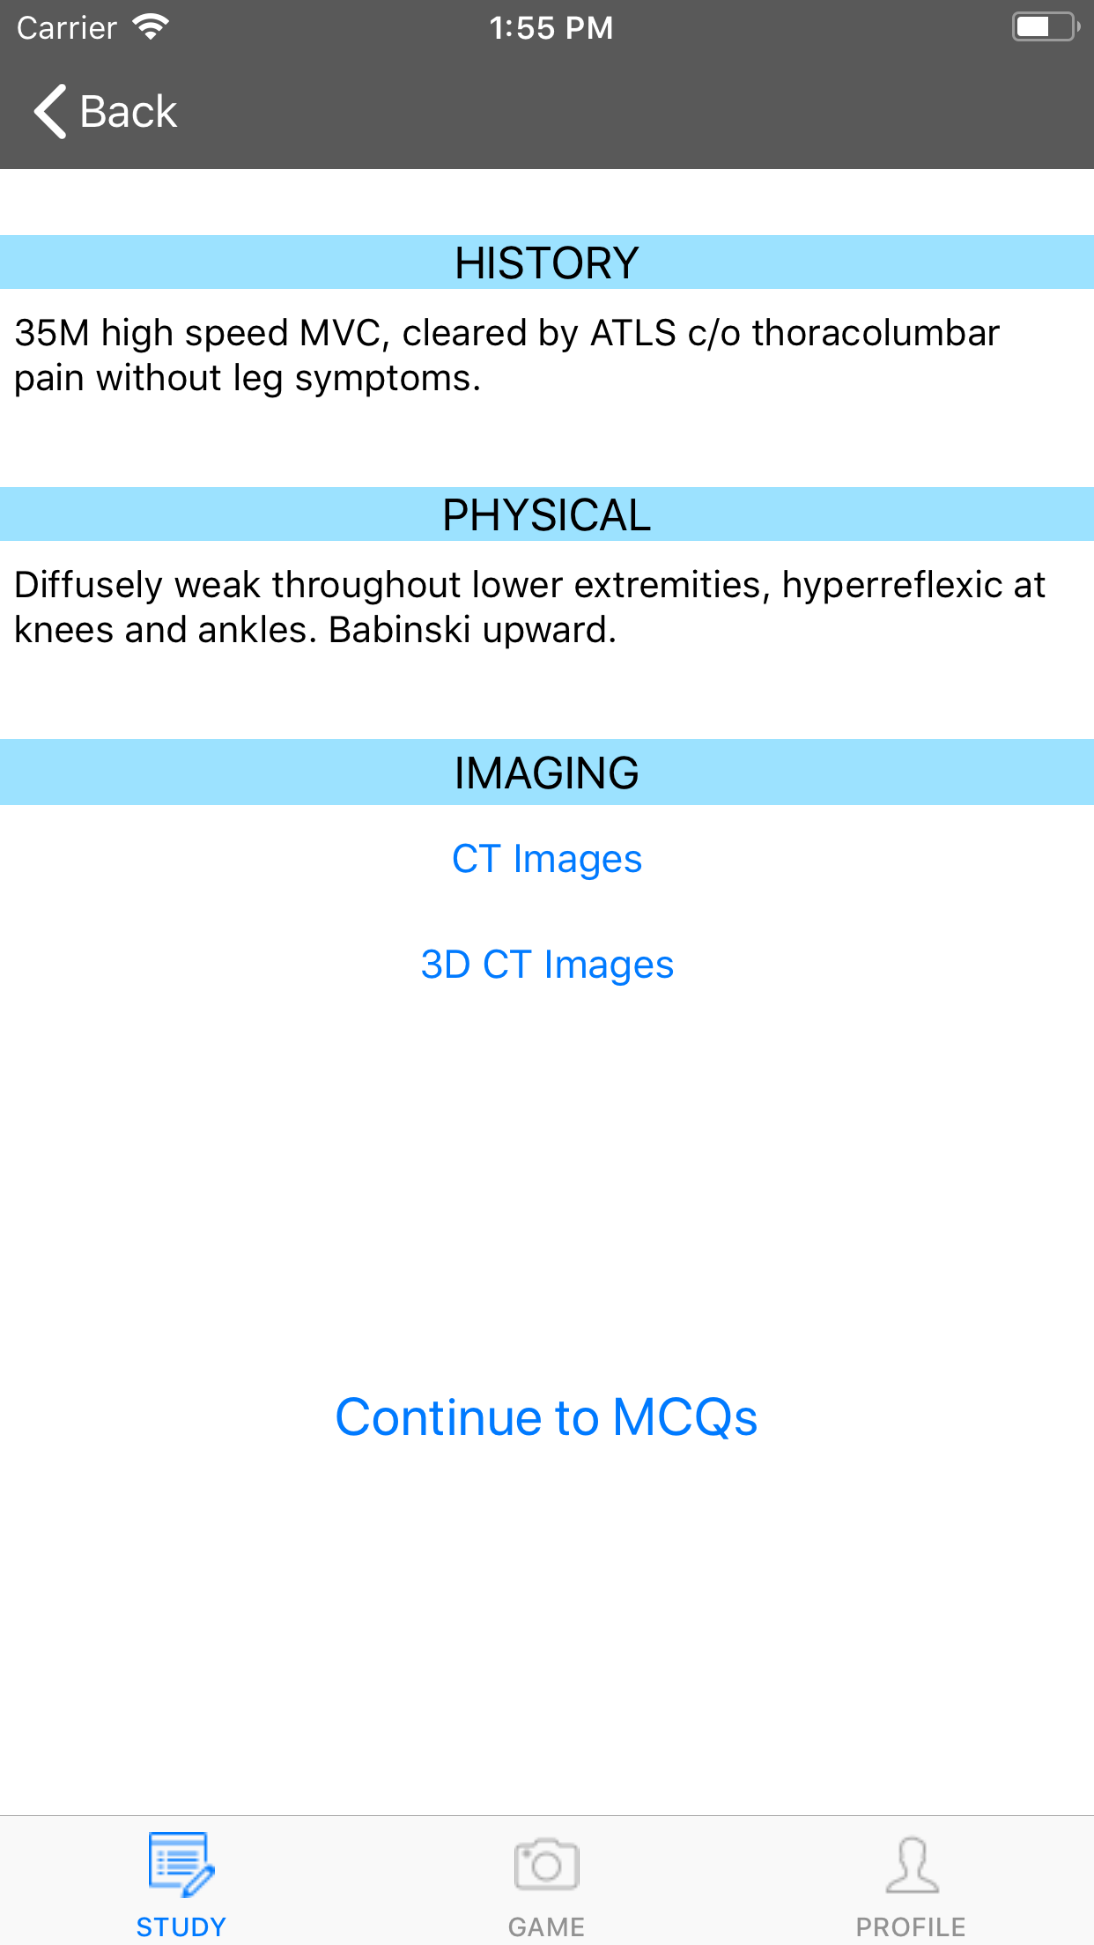
\includegraphics[width=0.4\textwidth, height=22cm]{cases.png}

\end{wrapfigure}
\large
Within the cases section, the user selects a case and is directed to a page that contains the patient's general history, information from their physical examination, and links to the pre-op CT images. This information will help the user answer the upcoming multiple choice questions. 
\end{block}

%----------------------------------------------------------------------------------------
%	Images
%----------------------------------------------------------------------------------------

\begin{block}{\LARGE Images}

\begin{wrapfigure}{L}{0.55\textwidth}
\centering
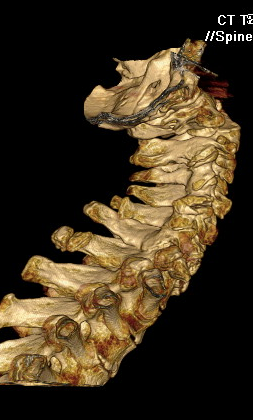
\includegraphics[width=0.5\textwidth, height=20cm]{ct-spine.png}
\end{wrapfigure}
\large
Spinal surgical cases often consist of 2D and 3D images saved after each patient undergoes CT or MRI scans. They are unique and valuable; even image manipulation software cannot design such realistic spinal deformity scans. Our team of medical surgeons anonymize the images and incorporate them into the medical cases mentioned above.
\newline
\end{block}

%----------------------------------------------------------------------------------------
%	Multiple Choice Questions
%----------------------------------------------------------------------------------------
\begin{block}{\LARGE Multiple Choice Questions}

\begin{wrapfigure}{R}{0.5\textwidth}
\centering
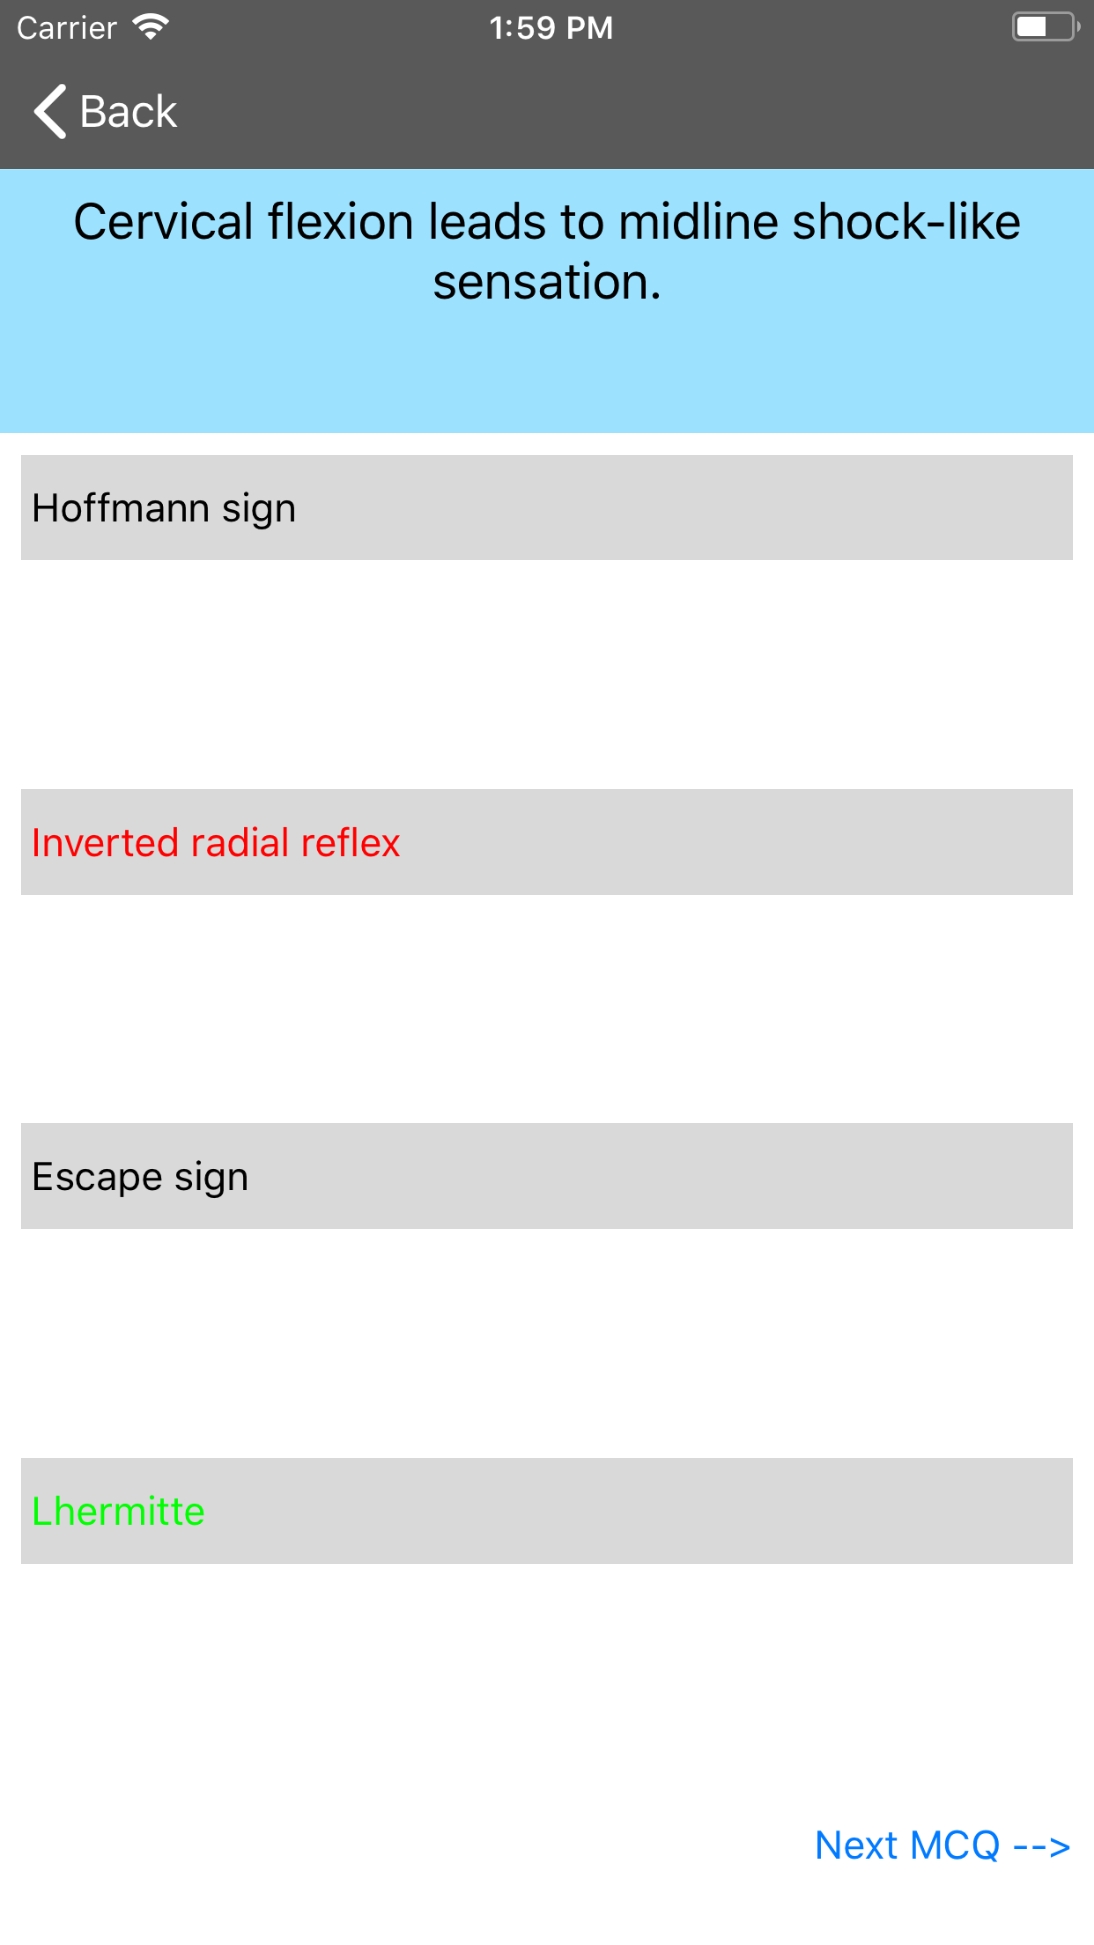
\includegraphics[width=0.4\textwidth, height=20cm]{mcq.png}

\end{wrapfigure}
\large
The multiple choice questions quiz users on their knowledge. Users will see a question and 4 options. If the user selects the correct answer, the option will turn green. If the user selects the wrong answer, the option will turn red, and the correct answer will turn green. The user will be able to immediately learn from their mistakes.

\end{block}

%----------------------------------------------------------------------------------------

\end{column} % End of the first column

\begin{column}{\onecolwid} % The first column

%----------------------------------------------------------------------------------------
%	Objectives
%----------------------------------------------------------------------------------------

\begin{alertblock}{\LARGE Objectives}

\large
Our project aims to provide users with real clinical scenarios and multiple choice questions that help prepare students for their medical exams. Additionally, our project allows medical students to practise performing procedures inside an augmented reality environment.

\end{alertblock}

%------------------------------------------------

\begin{figure}
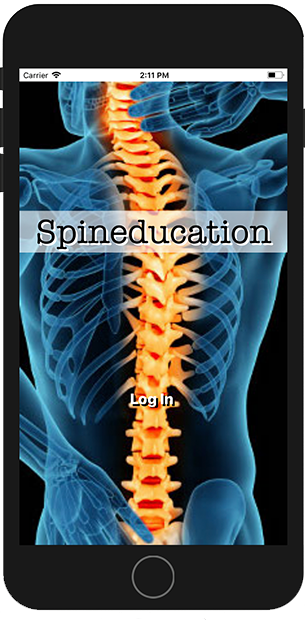
\includegraphics[width=30cm,height=50cm,keepaspectratio]{homescreen.png}
\end{figure}

%----------------------------------------------------------------------------------------

%----------------------------------------------------------------------------------------
%	Target Audience
%----------------------------------------------------------------------------------------

\begin{block}{\LARGE Target Audience}
\large
When it comes to hands-on experience, medical students have little opportunity to practice their skills in spinal surgery due to the intricate nature; as such, the user of a medical application like ours would be provided a simulated practice experience through an augmented reality game as well as theoretical knowledge through cases and multiple choice questions.
\end{block}

\end{column} % End of the first column

\begin{column}{\onecolwid} % The third column

%----------------------------------------------------------------------------------------
%	3D Models
%----------------------------------------------------------------------------------------


\begin{block}{\LARGE AR Surgery}

\begin{wrapfigure}{L}{0.6\textwidth}
\centering
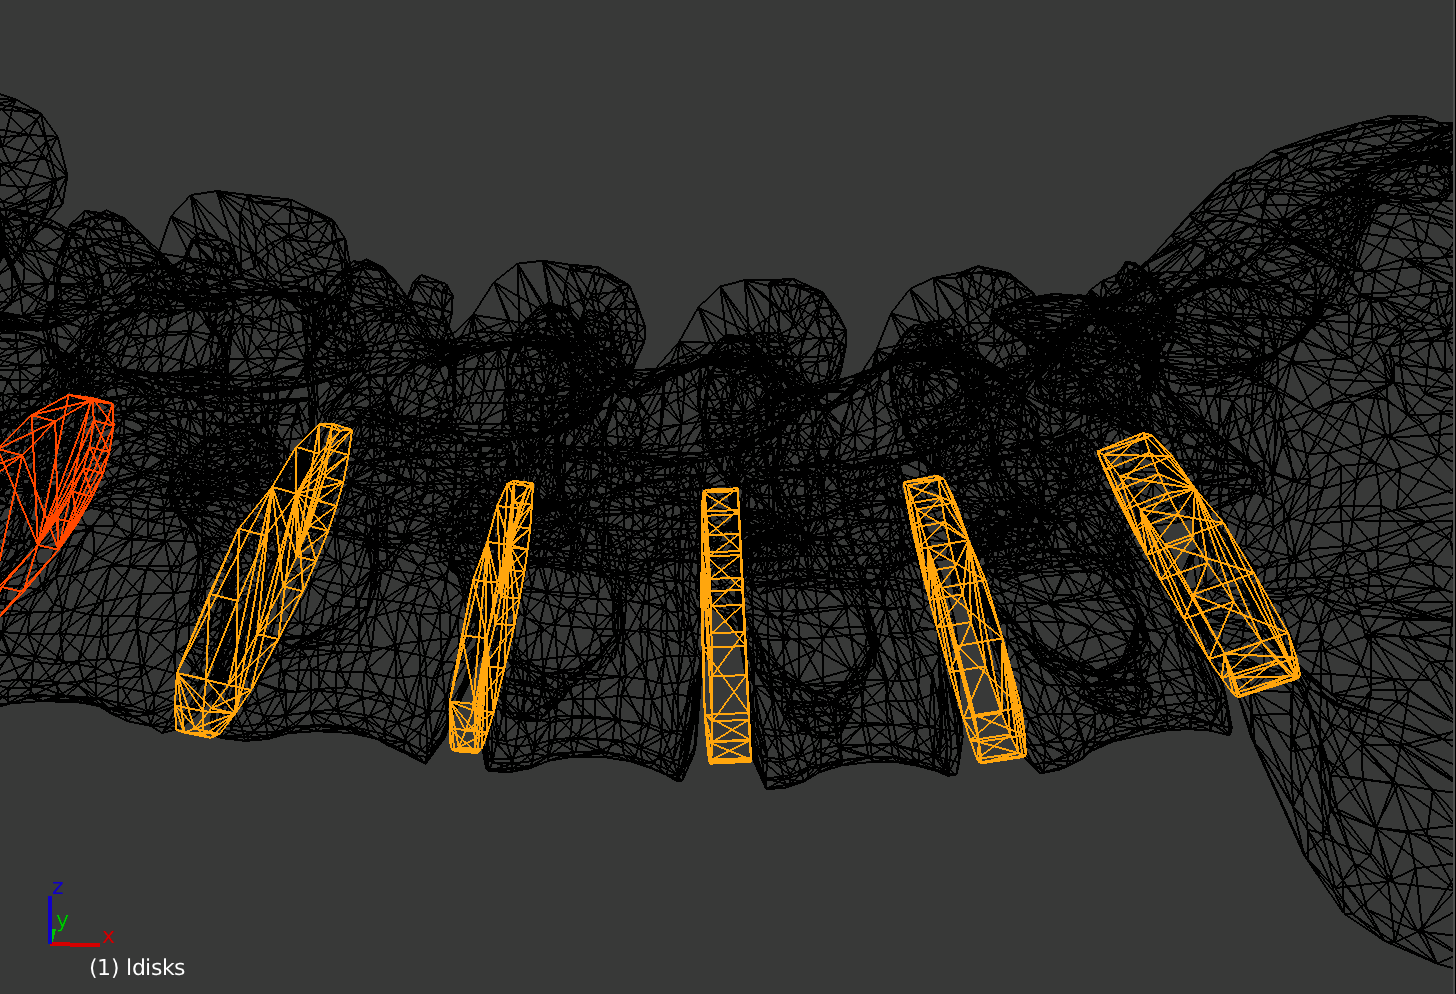
\includegraphics[width=0.5\textwidth,height=18cm]{spine.png}

\end{wrapfigure}
\large
The augmented reality component of the application uses blender to texture and manipulate a 3D model of the spine, helping ensure that the spine that iws superimposed in the user's environment has all necessary attributes to provide the most lifelike surgical experience.

\end{block}

%----------------------------------------------------------------------------------------
%	Trajectory
%----------------------------------------------------------------------------------------

\begin{block}{\LARGE Selecting Start Points and Trajectory}

\begin{wrapfigure}{R}{0.6\textwidth}
\centering
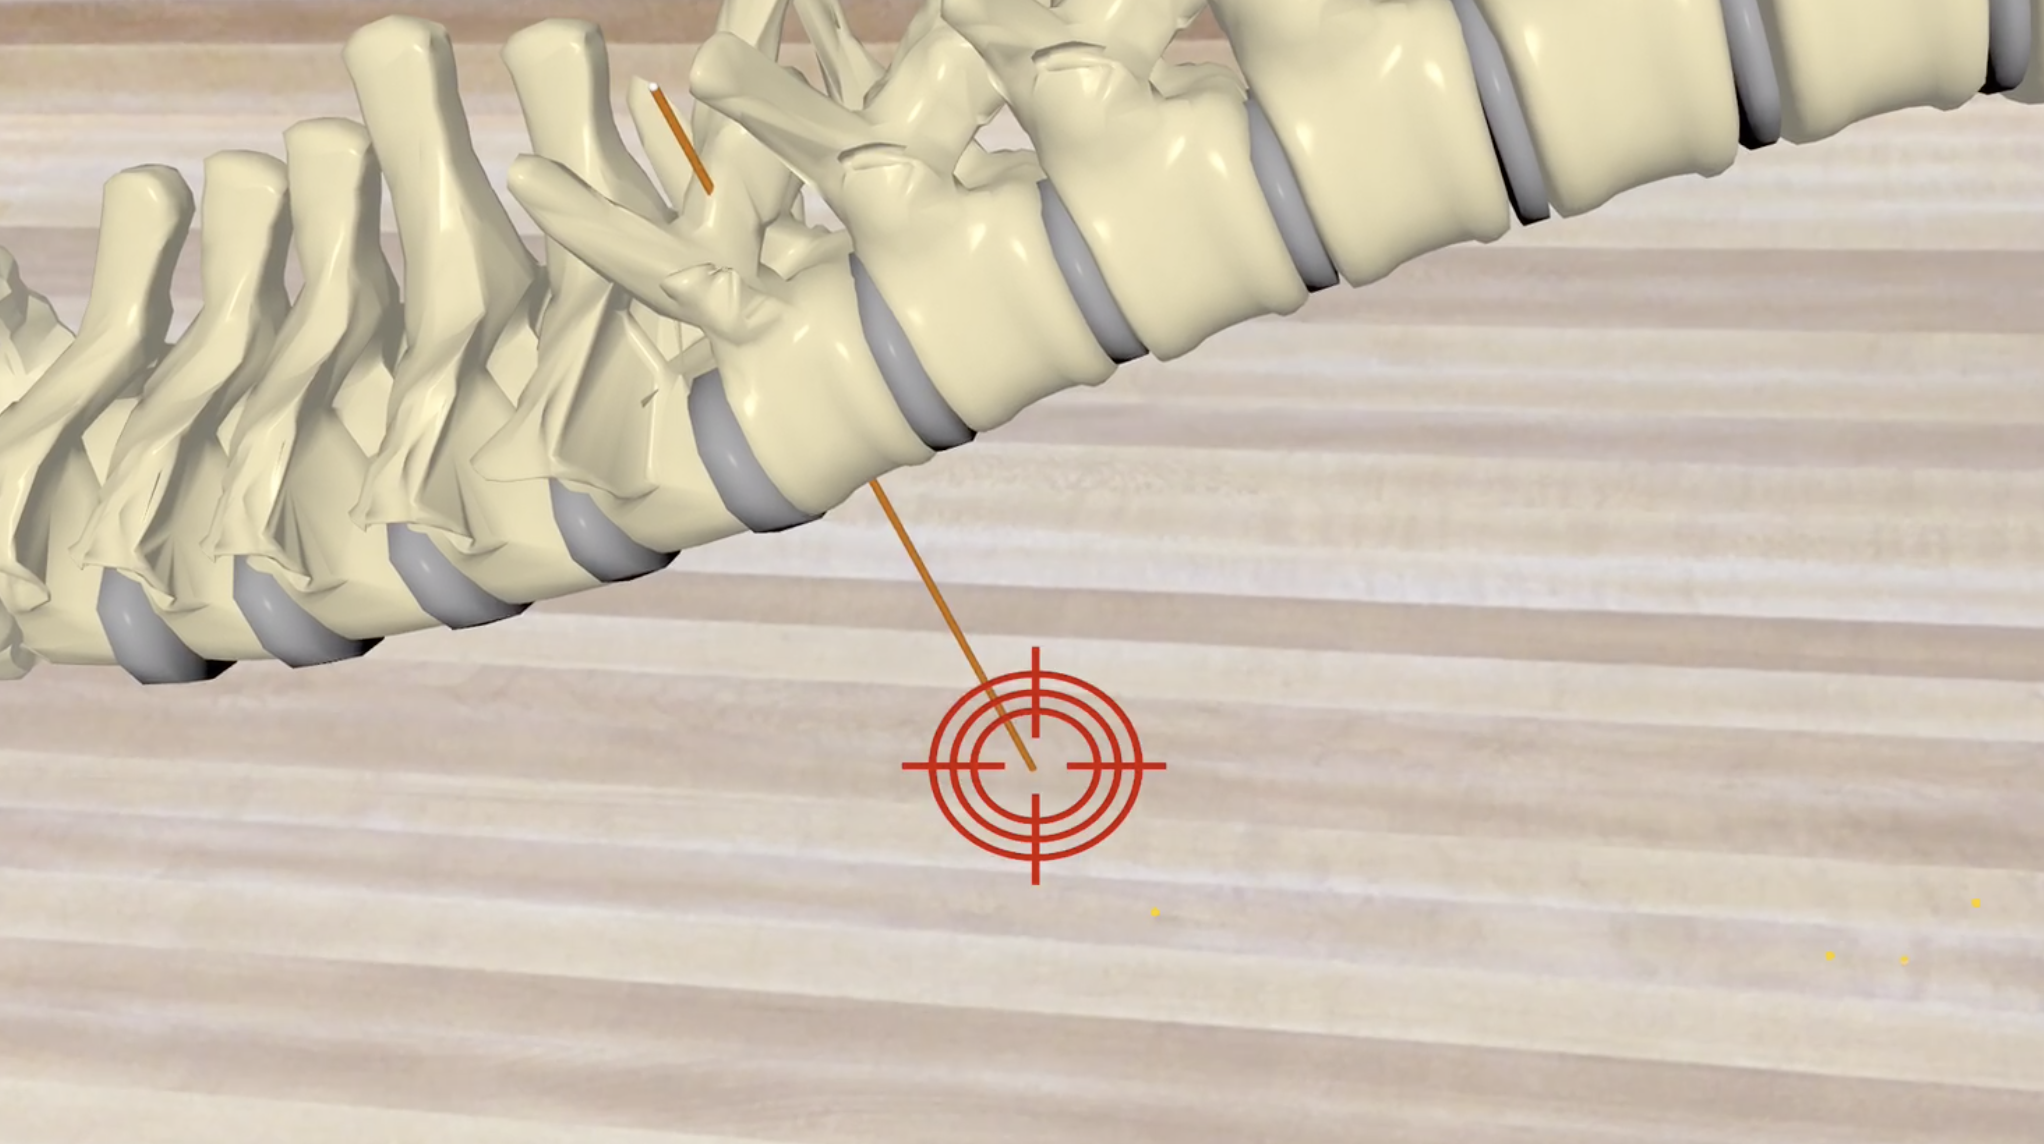
\includegraphics[width=0.5\textwidth, height=18cm]{trajectory.png}

\end{wrapfigure}

\large 
In order to simulate trajectory selection, when a pedicle start point is chosen, a line from the start point to the user appears; this allows the user to move the line according to the camera angle and select a trajectory with which they place the screw into the pedicle start point on the spine.

\end{block}

%----------------------------------------------------------------------------------------
%	Screws
%----------------------------------------------------------------------------------------
\begin{block}{\LARGE Placement of Screws}

\begin{wrapfigure}{L}{0.6\textwidth}
\centering
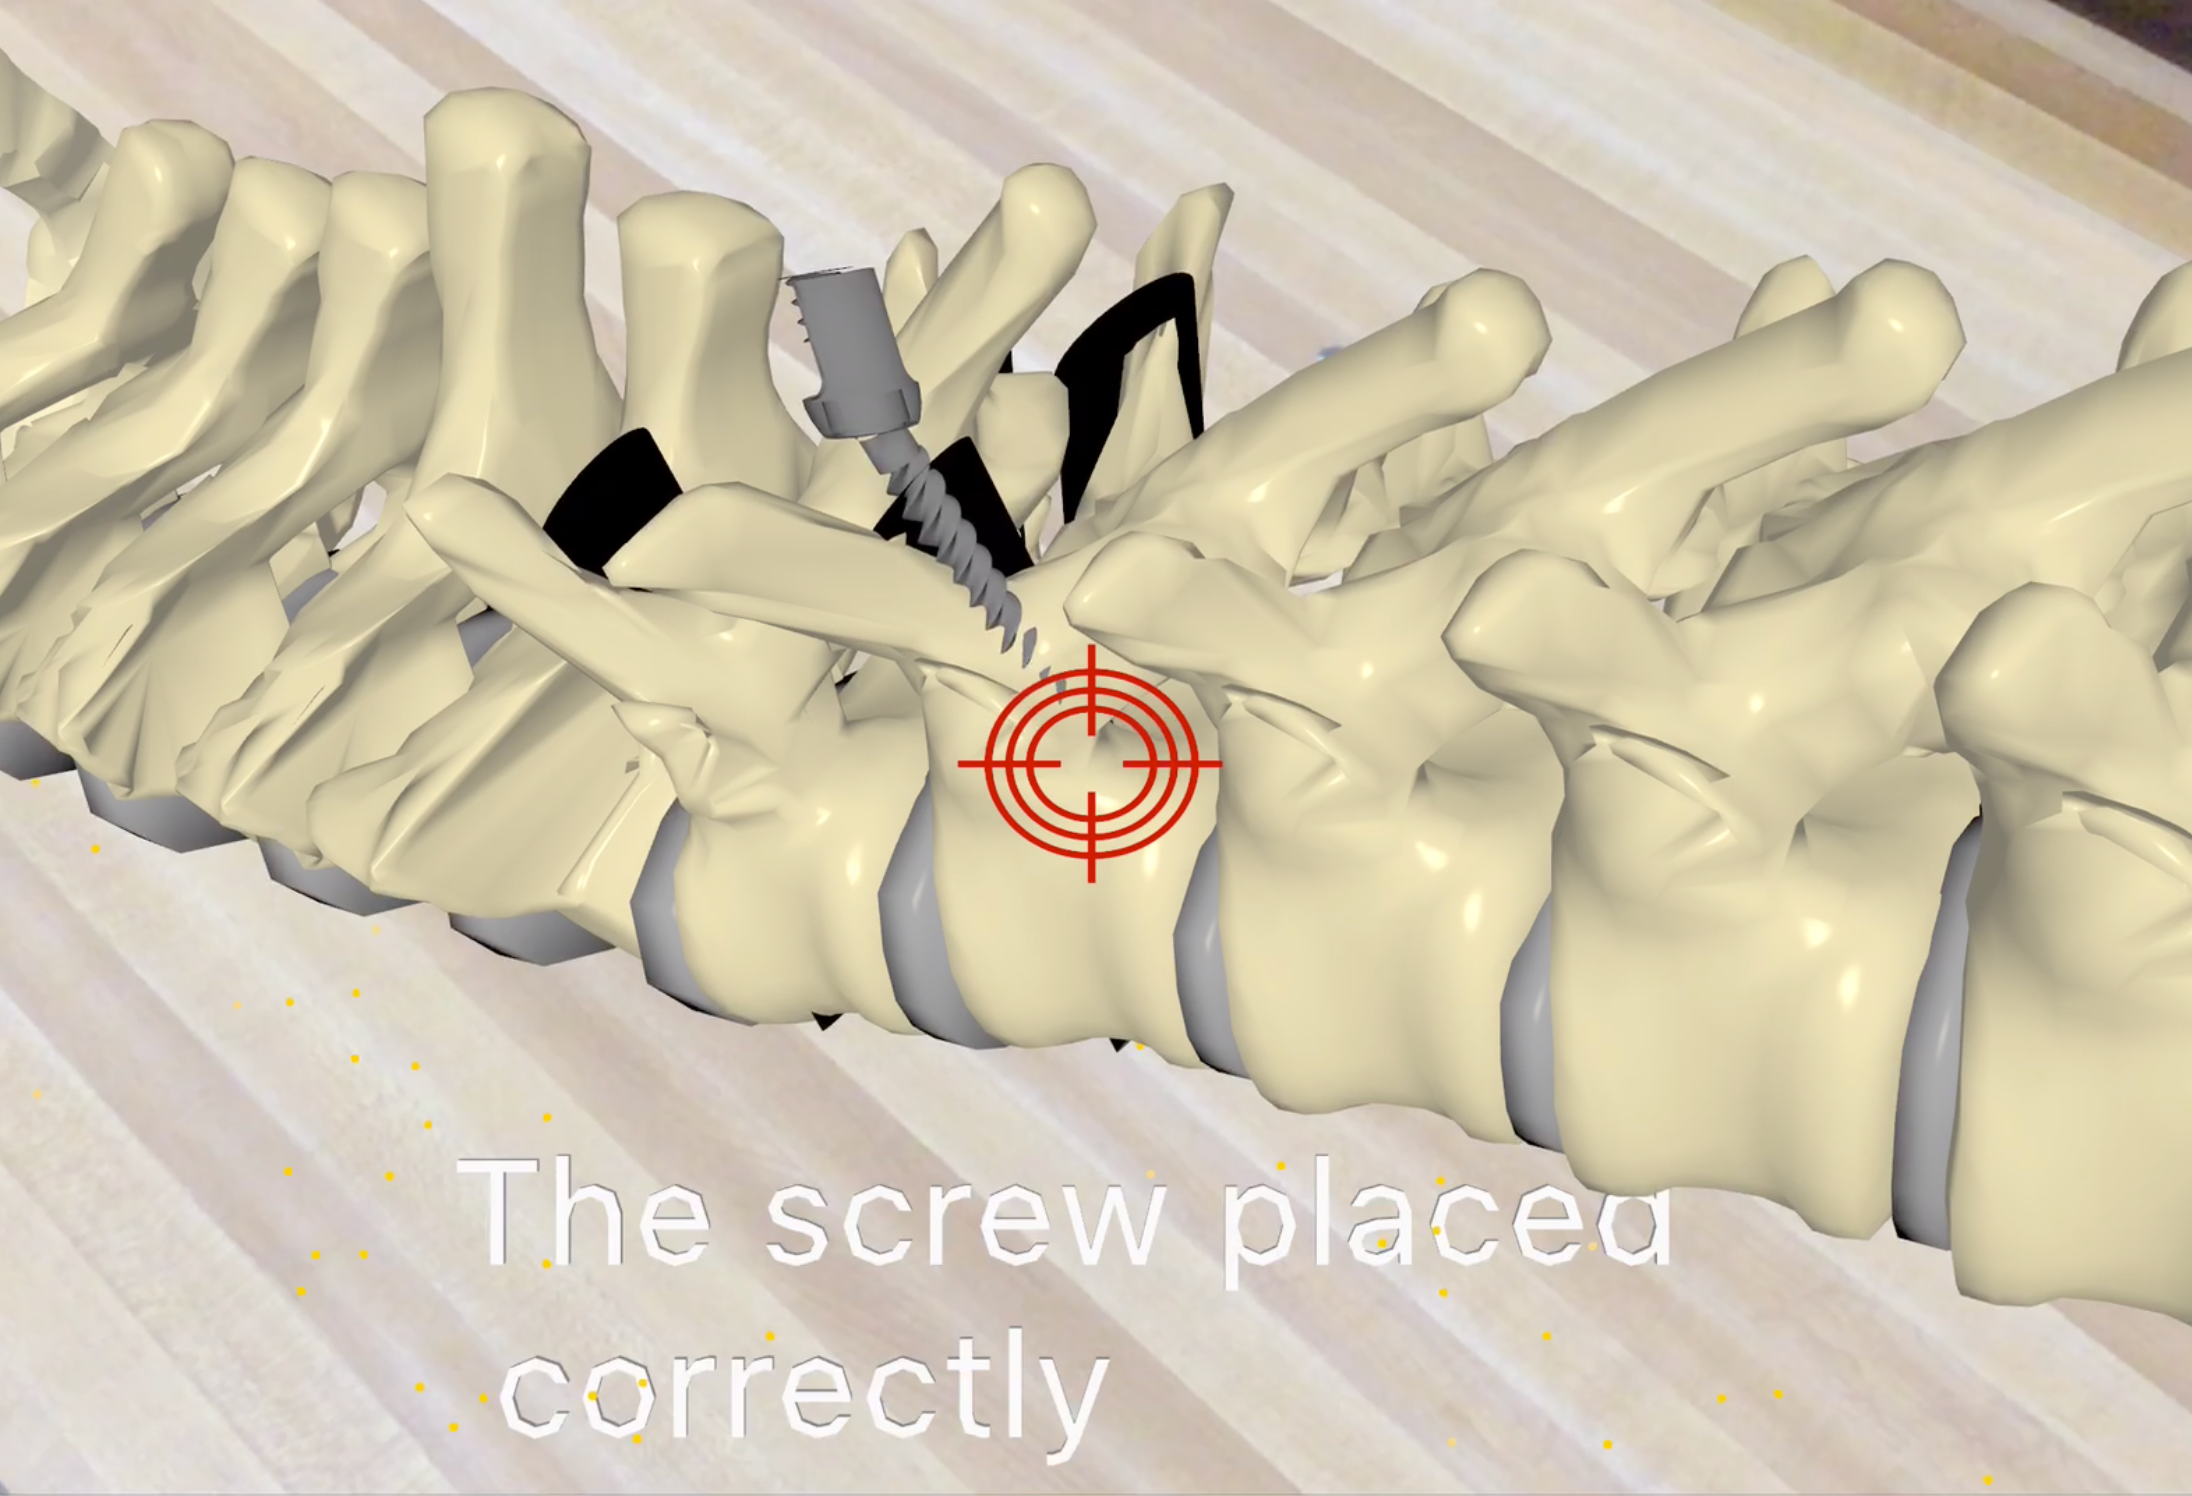
\includegraphics[width=0.5\textwidth,height=20cm]{screw.png}

\end{wrapfigure}
\large
Afterwards, the screw is placed using the selected position and by calculating the rotation angle from the camera. If the placement of the screw is within the designated pedicle start point, then the screw has been placed successfully.

\end{block}

%----------------------------------------------------------------------------------------

\end{column} % End of the third column

\end{columns} % End of all the columns in the poster

\end{frame} % End of the enclosing frame

\end{document}

